\subsubsection{Overfitting}\label{overfitting}

Knowing the basic functioning of a neural network using the forward-pass and backpropagation algorithm, it can be thought that if in each iteration of the model, the network trains and learns new patterns, the conclusion can be drawn that by carrying out infinite training, a perfect model can be obtained whose error has been minimised as much as possible and therefore the computed results are the expected ones. But this is not the case, having a wrong configuration of the network or training the network longer than necessary causes what is known as overfitting.
\newline


Overfitting is a well-known problem when training neural networks. It is usually caused by using a training that has been performed for a long time, causing the model to fit perfectly to the training data and somehow "memorize" the data and therefore, not know how to extrapolate and adapt to other cases. In other words, the $W$-matrix of all the layers is over-adjusted and thus, the model adapts perfectly to the input data producing that the model is not able to estimate a correct value when using an input vector that it had not seen before.

\begin{figure}[H]
    \centering
    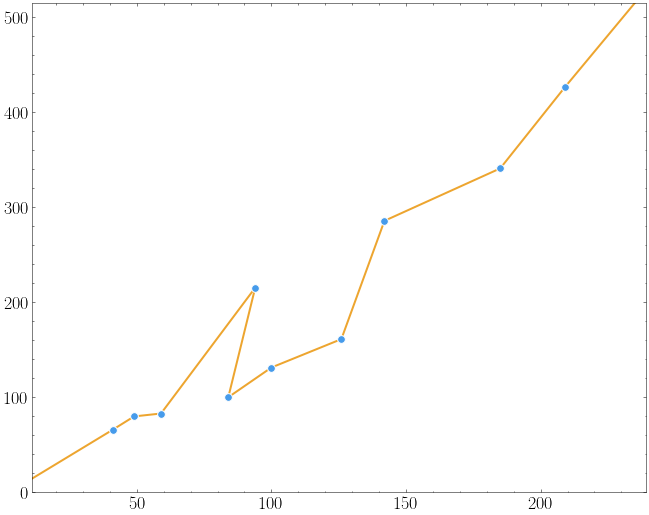
\includegraphics[width=12cm]{images/state-of-art/overfitting/overfitting.png}
    \caption{Example of overfitting in a linear regression.}
    \label{fig:basic_network}
\end{figure}

One of the fastest ways to know if a model is overfitting is by using a second dataset in addition to the training one. Normally, before creating a neural network, a pre-processing must be done. The original dataset is usually divided into three different datasets: training, validation and test. Obviously, the training dataset is used to train and adjust the parameters of the W matrices in an iterative way. On the other hand, there are the validation and test datasets that are used to evaluate different metrics. If the problem to be solved with the network is of regression type, some kind of error explained in section \ref{costfunction} is usually used as a metric, such as: \acrshort{mae}, \acrshort{mse} or Huber error. On the other hand, if the problem to be solved is a classification problem, precision is usually used as a metric.
\newline

If we see that the accuracy of the test data no longer improves, then we should stop training. Of course, strictly speaking, this is not necessarily a sign of overfitting. It could be that the accuracy of the test data and the training data stop improving at the same time. Even so, adopting this strategy will avoid overfitting.
\newline

At the end of each epoch, a subset of data from the training dataset and another subset from the validation dataset will be used. With these, the value of the selected metric will be calculated and two metrics will be obtained. These metrics can be compared between them. Two metrics that are similar indicate that the model is capable of extrapolating to other cases that it has not used for training. On the contrary, if the value associated to the training dataset is much better than the value associated to the validation dataset this may mean that the model may be suffering from overfitting. A training carried out without overfitting can be visualised in figure \ref{fig:overfitting}.
\newline

At the beginning of the training, as the network has not been trained and the parameters initialised randomly, the model will have quite bad metrics, i.e. if any error is being used, this value will be very high. On the other hand, if you are measuring the accuracy of the model, this value will be far from 100\%. These metrics will be equally bad for both datasets. As epochs occur during the training, the model will not be able to improve anymore and will start to memorise the data with which it is being trained from the training dataset causing the metric associated with the training to be almost perfect and the validation metric to get progressively worse. An example of an overfitting training can be seen as follows:
\newline

\begin{figure}[H]
    \centering
    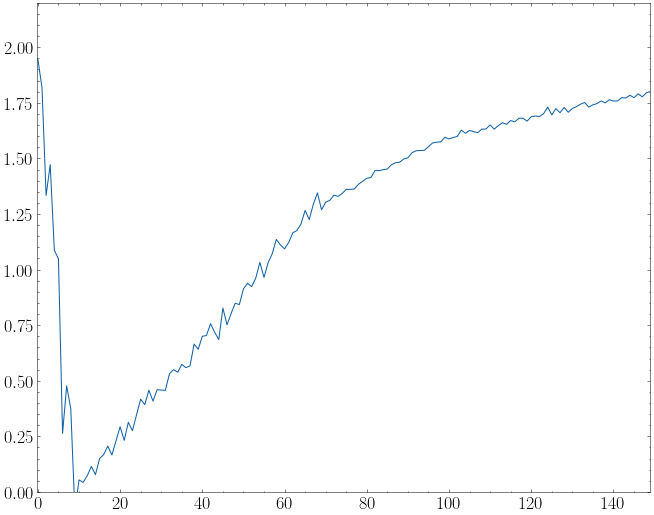
\includegraphics[width=12cm]{images/state-of-art/overfitting/overfitting-loss.png}
    \caption{Example of overfitting in a linear regression using an error as a metric.}
    \label{fig:overfitting}
\end{figure}

At the beginning of the training both metrics stop, until they reach approximately epoch 10, at which point the validation metric can be seen to gradually worsen. It is at this point that you can see that the network has an overfitting problem. Depending on the metric used, the overfitting can appear before or after, but it is a more complex issue that will not be explained in this paper.
\newline

There are still several techniques that will be explained below to avoid overfitting: 
\begin{itemize}
    \item Regularization L1 and L2:
    These are two methods that calculate a value known as a penalty that is added to the error and thus can penalise parameters with large values. If a neuron has large values it may be a sign that the neuron is trying to memorise. In fact, it is considered bad practice to let a small set of neurons in the network bear the greatest responsibility, i.e., their associated parameters are very large.
    \newline
    
On the one hand, you have L1 which is the sum of all the absolute values of $w$ and $b$. It is a linear penalty since the associated function is directly proportional to the parameters. The penalty L2 is the sum of all parameters $w$ and $b$ squared. It is a non-linear function and penalises with greater intensity the large values, unlike L1 that penalises much more in proportion to the small values because it is linear. This causes the model to become invariant to small input values and variant only to large values. Therefore, L1 is rarely used unless it is in combination with L2. Both functions are dependent on a value $\lambda$, with this value you can dictate how much impact L1 and L2 will have on the final error. Mathematically:
    
    \begin{align*}
         L_{1w} = \lambda \sum_m |w_m| &&  L_{2w} = \lambda \sum_m w^2_m \addtocounter{equation}{1}\tag{\theequation} \\ 
         L_{1b} =\lambda \sum_n |b_n| && L_{2b} = \lambda \sum_n b^2_n \addtocounter{equation}{1}\tag{\theequation}
    \end{align*}
    
The final error is given by the simple sum of the error calculated by the cost function and L1 with L2:
    \begin{equation}
        c_T = c + L_{1w} + L_{1b} + L_{2w} + L_{2b}
    \end{equation}

As regularization is used for the calculation of $c$, it is necessary to know its derivative in order to use back-propagation. The cost derivative is as follows:
    
    \begin{equation}
        \frac{\partial c_T}{\partial w^{L_i}} = c' + L'_{1w} + L'_{1b} + L'_{2w} + L'_{2b}
    \end{equation}
    
The L1 and L2 derivatives are as follows:
\begin{align*}
     L'_{1w} = \lambda \begin{cases} 1,& \text{si } w_m > 1\\ -1,& \text{si } w_m < 1\end{cases} && L'_{2w} =  2\lambda w_m \addtocounter{equation}{1}\tag{\theequation} \\ 
     L'_{1b} =  \lambda \begin{cases} 1,& \text{si } b_n > 1\\ -1,& \text{si } b_n < 1\end{cases} && L'_{2b} = 2\lambda b_n \addtocounter{equation}{1}\tag{\theequation}
\end{align*}
    
    \item Dropout \label{dropout}: Using this technique, in each iteration of the training the network is modified. Let's suppose that you have an input $x$ and the desired value $y$. Ordinarily, you would train by propagating $x$ forward through the network, and then propagating it backward to determine the contribution to the gradient. With dropout, this process is modified. It starts by randomly (and temporarily) removing a percentage of the hidden neurons in the network, while leaving the incoming and outgoing neurons unchanged. The neurons that have been deleted will be "ghost" neurons for that epoch:
    
    \begin{figure}[H]
        \centering
        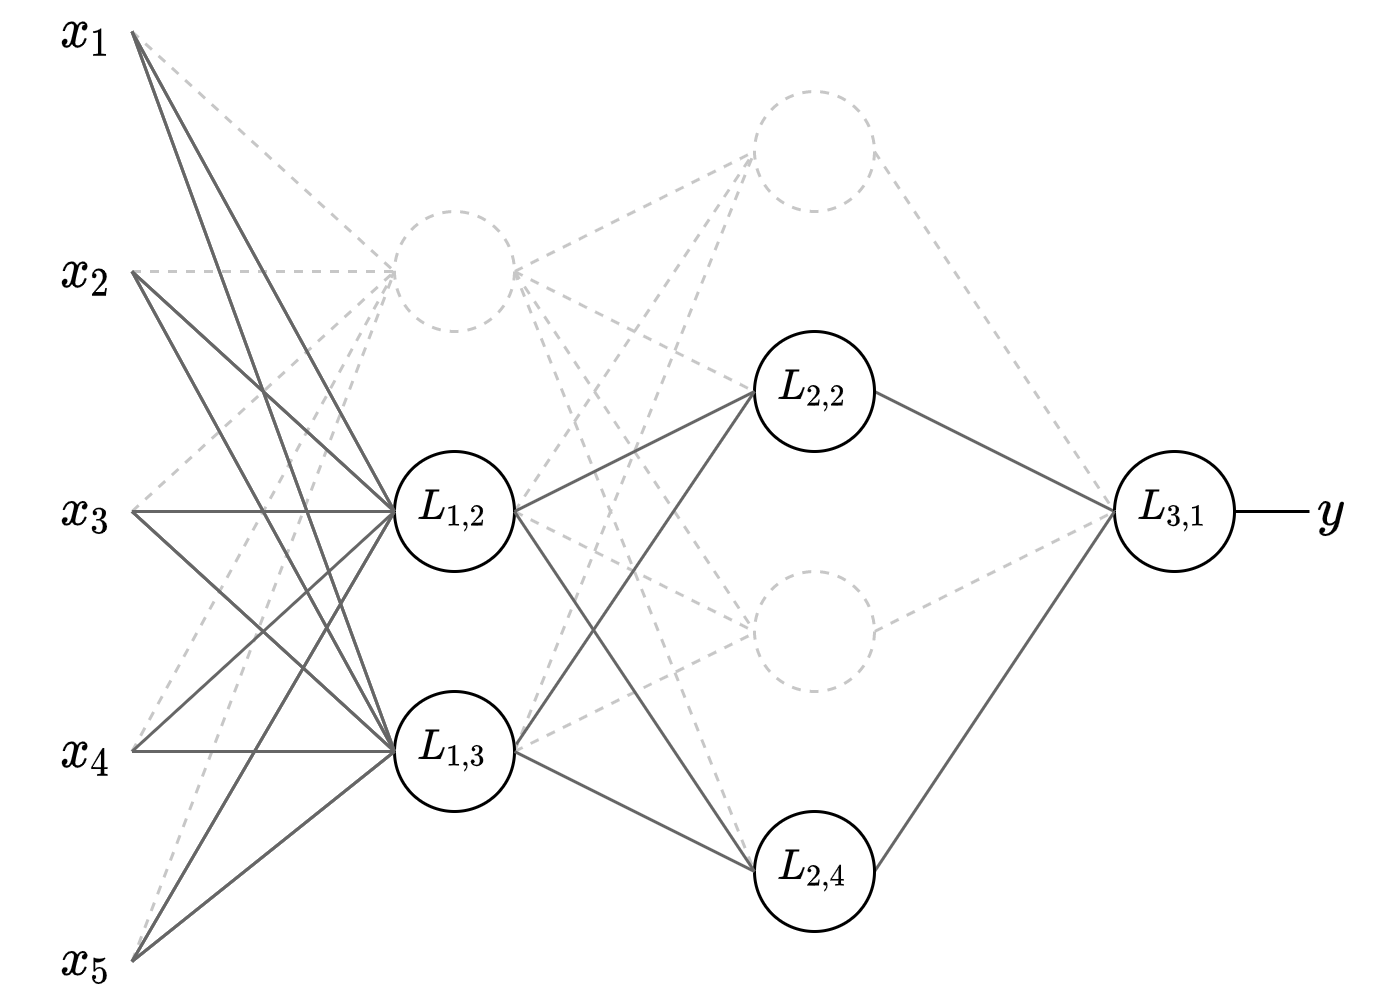
\includegraphics[width=12cm]{images/state-of-art/overfitting/dropout-1.png}
        \caption{Dropout applied to a network with $50\%$ probability}
        \label{fig:basic_network}
    \end{figure}
    
    
    Once the process of forward propagation and backpropagation has been completed, a new epoch will begin by randomly eliminating a set of neurons. In short, for each iteration, a subset of the neurons will be eliminated according to a given percentage.
    \newline
    
    By repeating this process throughout the training phase, the network will learn $W$-matrixes that will have been learned under conditions where a subset of the hidden neurons was removed. When the whole network is actually executed, it will mean that the number of active neurons will be higher. Therefore, it will be compensated by reducing the proportional part with those that were entered. For example, using a percentage equal to $50$, the values of $W$ will be half of what the gradient has calculated.
    
    \item Selection of an iterative learning rate: This technique is based on the study of various learning rates depending on the epoch of the training. A set of values is usually given in an orderly fashion between a minimum and a maximum. Each value of this interval will be a learning rate for different epochs and it will be possible to study their behaviour and see if the descent of the gradient is capable of converging.
    \newline
    
    If it can converge, the results obtained will be those expected, making the cost function progressively smaller. On the contrary, if the learning rate is very low or very high, it will cause that the descent of the gradient cannot converge resulting in the result of the cost function being irregular and generally worsening the model.

\end{itemize}

